\documentclass[brudnopis]{xmgr}
% \documentclass[openright]{xmgr}
\usepackage[utf8]{inputenc}
\usepackage{caption}
\usepackage{color}
\usepackage{float}
\usepackage{graphicx}
\usepackage{parskip}
\usepackage[dvipsnames]{xcolor}
\usepackage{csquotes}
\usepackage{listings}
\usepackage{hyperref}

\graphicspath{ {images/} }

% Odległości między paragrafami oraz wcięcia
\setlength{\parskip}{1em}
\setlength{\parindent}{3em}

% Środowisko bez page-breaków, z zachowanymi odległościami między paragrafami oraz wcięciami
% NOTE: Póki co nie używane w treści licencjatu
\newlength{\currentparskip}
\newlength{\currentparindent}
\newenvironment{nopgbreak}
  {\setlength{\currentparskip}{\parskip}
   \setlength{\currentparindent}{\parindent}
   \begin{minipage}{\textwidth}
   \setlength{\parskip}{\currentparskip}
   \setlength{\parindent}{\currentparindent}
  }
  {\end{minipage}}

% Specjalne oznaczenia
\newcommand{\name}[1]{\textbf{\textcolor{NavyBlue}{#1}}}
\newcommand{\todoadrian}{\textbf{\textcolor{red}{<< TO MIEJSCE WYPEŁNIA ADRIAN >>}}}
\newcommand{\todomateusz}{\textbf{\textcolor{red}{<< TO MIEJSCE WYPEŁNIA MATEUSZ >>}}}

% Podświetlanie składni C#
\definecolor{bluekeywords}{rgb}{0.13,0.13,1}
\definecolor{greencomments}{rgb}{0,0.5,0}
\definecolor{redstrings}{rgb}{0.9,0,0}
\lstset{language=[Sharp]C,
captionpos=b,
%numbers=left, %Nummerierung
%numberstyle=\tiny, % kleine Zeilennummern
frame=lines, % Oberhalb und unterhalb des Listings ist eine Linie
showspaces=false,
showtabs=false,
breaklines=true,
showstringspaces=false,
breakatwhitespace=true,
escapeinside={(*@}{@*)},
commentstyle=\color{greencomments},
morekeywords={partial, var, value, get, set},
keywordstyle=\color{bluekeywords},
stringstyle=\color{redstrings},
basicstyle=\ttfamily\small,
}

% Dane licencjatu
\wersja   {wersja wstępna [\ymdtoday]}
\author   {Mateusz Kleina, Adrian Podlawski}
\nralbumu {231\,068}
\title    {Sieciowa fabularna gra komputerowa - The Trinity}
\date     {2017}
\miejsce  {Gdańsk}
\opiekun  {dr W. Bzyl}


\begin{document}

% Strona tytułowa
\keywords{Gra, RPG, Multiplayer, Unity, PhotonUnityNetwork}

\begin{abstract}
\section{Streszczenie}
Zaimplementowaliśmy wieloosobową grę, która bazuje na silniku graficznym Unity. 
Serwer, z którym łączą się gracze znajduje się w chmurze, którą oferuje Framework Photon Unity 3D Networking. 
Mapa została utworzona dzięki technologii Unity, która pozwala na dowolne kształtowanie terenu.
Krajobrazy oraz budynki zostały pobrane z Assets Store oraz odpowiednio zmodyfikowane tak, by spełniały wymagania gry. 
Wszystkie skrypty odpowiadające za sterowanie postaci, łączenie z serwerem, czy walkę z przeciwnikiem, zostały utworzone na potrzeby gry w obiektowym języku programowania C Sharp.
W trakcie rozwijania aplikacji, pliki były przechowywane we wspólnym repozytorium na stronie Github.com. 
Początkowym założeniem naszej pracy było utworzenie gry wieloosobowej, której świat jednocześnie będzie mogła eksplorować trójka graczy. Każdy z nich sterowałby inną, unikatową postacią. 
Gra miała posiadać przykładowe misje oraz stanowić fundament do dalszego jej rozwoju, w późniejszym czasie na tle fabularnym. Wszystkie powyższe założenia udało nam się zrealizować. 
W poniższej pracy przedstawimy ze szczegółami cały proces powstawania naszej produkcji. 
\end{abstract}

\maketitle

\include{wstep_i_opis}

\chapter{Projektowanie oraz przygotowanie środowiska}
\section{Projekt Terenu}
Projektowanie naszego terenu zaczęliśmy od lokacji startowej, czyli miasta, w którym rozpoczyna się gra. 
Stworzyliśmy spustoszone miasto, które miało oddawać klimat, w jakim został osadzony cały projekt. 
\begin{figure}[H]
	\center
	\includegraphics[width=8cm]{scena.png}
	\caption{Początkowa lokacja na scenie, w której bohaterowie rozpoczynają przygodę}
\end{figure}
Na początku rozgrywki napotkamy kilku przeciwników oraz przerażoną kobietę, która wprowadzi nas w świat gry.  
Postaci kierowane przez graczy posiadają określoną rolę, dlatego dalsza część mapy została zaprojektowana z myślą o specjalnych umiejętnościach każdego z nich.
Po drodze możemy spotkać niezliczone grupy przeciwników oraz przeszkody w postaci ukształtowania terenu, które możemy pokonać tylko przy pomocy jednego z bohaterów.
Przez resztę rozgrywki poruszamy się krętą ścieżką, która prowadzi do oazy.
Jest to płaski otwarty teren, na którym bohaterowie będą mogli stoczyć ostateczną walkę ze źródłem swoich problemów.
\begin{figure}[H]
	\center
	\includegraphics[width=8cm]{scena2.png}
	\caption{Przykładowa przeszkoda w postaci ukształtowania terenu}
\end{figure}
\subsection{Projekt Postaci}
Postaci zostały utworzone przy pomocy strony www.mixamo.com. Wybraliśmy modele, w których przeważają ciemne kolory, a ich charakteryzacja współgra z mrocznym klimatem otoczenia. 
Następnie do każdej postaci zostały dopasowane animacje, które mogliśmy wykorzystać podczas procesu implementacji.
Ostatnim krokiem było wybranie szczegółów takich jak ilość klatek na sekundę (FPS) z jaką mają być wyświetlane animacje. 
Po wykonaniu powyższych czynności pakiet postaci mógł zostać pobrany, a następnie dołączony do projektu. 
\section{Projekt systemu mulitplayer}
Do utworzenia systemu Multiplayer został użyty Framework Photon Unity 3D Networking często nazywany PUN. 
Photon udostępnia również chmurę, na której znajduje się nasza aplikacja, dzięki temu nie jest wymagane użycie innego, zewnętrznego serwera. 
\begin{figure}[H]
	\center
	\includegraphics[width=\textwidth]{maszyny.png}
	\caption{Serwery udostępniane przez framework Photon, na których znajdują się nasze środowiska testowe oraz produkcyjne}
\end{figure}
Gracze po włączeniu gry automatycznie dołączają do rozgrywki. Maksymalnie do jednej rozgrywki może połączyć się trzech graczy. Jeżeli do serwera dołączy czwarty gracz, zostanie utworzony kolejny pokój gry, a wszyscy kolejni użytkownicy będą mogli się z nim połączyć, dopóki nie zostanie osiągnięty limit osób. 
Każda postać jest unikatowa i poszczególny gracz może sterować tylko jedną z nich. Jeśli jeden gracz opuści grę, kolejny po dołączeniu zajmie jego miejsce. 
\subsection{Instalacja niezbędnych narzędzi}
Pierwszym krokiem było zainstalowanie Unity – silnika, na którym utworzona została nasza gra. 

Do tworzenia oraz edycji skryptów, używaliśmy dwóch środowisk, Visual Studio IDE oraz Visual Studio Code. 

Dla usprawnienia wspólnej pracy użyliśmy rozproszonego systemu kontroli wersji GIT. Korzystaliśmy zarówno z programu używając wiersza poleceń jak i aplikacji GitHub Desktop.

Podczas pracy nad naszym projektem często działaliśmy na tych samych, obszernych plikach np. w przypadku edycji mapy, po której poruszają się gracze. 
Przez to podczas łączenia naszych zmian często dochodziło do konfliktów w kodzie, których system kontroli wersji nie mógł sam rozwiązać. 
W tym wypadku niezbędne okazało się narzędzie UnityYAMLMerge, które znacznie usprawniło łączenie dwóch kopii, bez konieczności manualnego rozwiązywania konfliktów.

\chapter{Implementacja}
\section{Budowa terenu}\label{sec:budowa_terenu}
Budowa podstawowej mapy gry jest stosunkowo nieskomplikowanym procesem, dzięki czemu mogliśmy się tutaj skupić głównie na projektowaniu dróg, rozłożeniu obiektów i kształtowaniu mapy na potrzeby rozgrywki.

\subsection{Przygotowanie terenu}

    Do przygotowania terenu został użyty specjalnie do tego przeznaczony typ obiektu 3D o nazwie \name{Terrain}. Po utworzeniu takiego obiektu w hierarchii obiektów na ekranie ukaże się nieoteksturowana płaszczyzna.

    \begin{figure}[H]
    \includegraphics[width=\textwidth]{teren_1.png}
    \caption{Płaszczyzna terenu}
    \end{figure}

\subsection{Formowanie kształtu} 

    Na tak przygotowanej płaszczyźnie uformowane zostały nierówności przy użyciu palety narzędzi terenu. Używając opcji \name{Raise / Lower Terrain} utworzone zostały wypiętrzenia nadające kształt mapie gry. Charakter wypiętrzeń dostosowany został używając odpowiedniego pędzla z panelu \name{Brushes}, natomiast promień zniekształceń oraz siła efektu za pomocą parametrów kolejno \name{Brush Size} oraz \name {Opacity}.

    \begin{figure}[H]
    \includegraphics[width=\textwidth]{teren_2.png}
    \caption{Modelowanie nierówności terenu}
    \end{figure}

\subsection{Nakładanie tekstur}

    Kolejnym krokiem było utworzenie tekstury służącej do nadaniu naszemu terenowi koloru oraz faktury. Do tego celu pobrane zostały odpowiednie tekstury z wbudowanego sklepu assetów \name{Asset Store}. Assety są rodzajem pakietów zawierających różnorakie obiekty, skrypty oraz tekstury, dostępne do pobrania z serwerów Unity.

    Po pobraniu odpowiedniej tekstury trawy, zostaje ona zaimportowana do folderu \name{Assets} znajdującego się w głównym katalogu projektu.

    Po wybraniu narzędzia \name{Paint Texture} ukazuje się panel \name{Textures} pozwalający na skonfigurowanie używanej przez narzędzie tekstury. Znajduje się tam przycisk \name{Edit Textures...} po kliknięciu którego otwiera się okno konfiguracyjne tekstury pozwalające na wybór tekstury podstawowej oraz tekstury przechowującej dane o chropowatościach. Po skonfigurowaniu tekstur i nałożeniu ich na teren, całość prezentuje się następująco.

    \begin{figure}[H]
    \includegraphics[width=\textwidth]{teren_3.png}
    \caption{Nakładanie tekstur na mapę terenu}
    \end{figure}

\subsection{Rozmieszczanie obiektów}

    Kolejnym krokiem w tworzeniu świata gry było umieszczenie na mapie sprefabrykowanych wcześniej obiektów (tzw. \textit{Prefabs}, o tym później). Wszystkie obiekty użyte w pracy są dostępne za darmo w bibliotece obiektów Unity (\name{Asset Store}). Po pobraniu, obiekty znajdują się w podfolderze \name{Prefabs} zainstalowanej paczki. Obiekty umieszcza się na mapie metodą przeciągnij-upuść, dostosowując ich koordynaty używając narzędzi transformacji dostępnych w pasku narzędzi znajdującym się w górnej części okna edytora.

    \begin{figure}[H]
    \includegraphics[width=\textwidth]{teren_obiekty.png}
    \caption{Umieszczanie obiektów na mapie}
    \end{figure}

    % Szczegóły kolizji w sekcji~\ref{sec:fizyka} na stronie~\pageref{sec:fizyka}

\subsection{Oddziaływanie terenu na inne obiekty}

    Kluczowym elementem tworzenia mapy świata gry są takie elementy jak oddziaływanie na postacie ograniczeń nachylenia terenu typu wzgórza, drzewa, czy budynki, uniemożliwiających dostanie się w niektóre miejsca. Unity w celu uproszczenia obliczeń posiada możliwość wygenerowania uproszczonej mapy dróg (tzw. \textit{NavMesh}) na bazie modelu terenu, pozwalającej na dynamiczne omijanie przeszkód przez wroga (o tym później w sekcji \ref{sec:poruszanie_wrogow} na stronie \pageref{sec:poruszanie_wrogow}).

    Aby utworzyć taką mapę, należy przejść do zakładki \name{Navigation}, gdzie w panelu \name{Bake} znajduje się lista parametrów dotyczących maksymalnego kąta nachylenia terenu, czy maksymalnej wysokości uskoku, którą obiekty sterowane przez komputer mogą pokonać.

    \begin{figure}[H]
    \center
    \includegraphics[width=6cm]{teren_obiekty2.png}
    \caption{Parametry mapy dróg}
    \end{figure}

    Po ustaleniu parametrów i kliknięciu przycisku \name{Bake}, mapa zostaje wygenerowana, natomiast w oknie widoku sceny, obszary dostępne do przemierzania oznaczone zostają niebieskim kolorem. Operację można powtarzać do uzyskania optymalnych efektów.

    \begin{figure}[H]
    \center
    \includegraphics[width=9cm]{teren_obiekty3.png}
    \caption{Poprawnie wygenerowany \textit{NavMesh}}
    \end{figure}

    Tak przygotowana mapa posłużyła nam do projektowania dalszej części gry.

    % Każdy obiekt utworzony w Unity posiada paletę komponentów. Komponenty pozwalają na określanie właściwości obiektów, takich jak rozmiar, pozycja, czy masa. Komponentami są również skrypty, pozwalające na określenie interacji obiektu z zewnętrznym światem (np. zdarzenie \textit{OnCollisionEnter}).
\section{Tworzenie Postaci}
Po zaprojektowaniu postaci dołączyliśmy je do naszego folderu z projektem. Żeby nasza postać pojawiła się na mapie, musimy ją przeciągnąć na wcześniej utworzoną scenę. Tak oto otrzymaliśmy nieruchomy model naszego maga. Aby upewnić się, że jest on poprawnie ulokowany, możemy sprawdzić zakładkę Hierarchy, gdzie znajdziemy listę wszystkich dostępnych obiektów na mapie. 

W naszym wypadku nie możemy jednak umieścić postaci od razu w rozgrywce, gdyż nie będzie mogła ona być poprawnie sterowana przez danego gracza. Żeby system Multiplayer działał sprawnie, musimy stworzyć tak zwanego „Prefaba”, czyli obiekt w grze, który ma pewne właściwości, może zostać wielokrotnie użyty, lub pojawić się np. w momencie zalogowania gracza do gry. W tym celu musimy przeciągnąć nasz obiekt, który ma zamienić się w typ Prefab z listy Hierarchy, do naszego folderu (W tym przypadku jest to folder Assets). Teraz w celu ulokowania naszych magów na mapie, wystarczy przeciągnąć obiekt z rozszerzeniem .prefab na naszą scenę. Przy umieszczaniu takich samych obiektów Unity automatycznie będzie dodawało do naszej nazwy numer obiektu np. Wizard (1). 
\begin{figure}[H]
	\center
	\includegraphics[width=\textwidth]{prefab.png}
	\caption{Ręczne rozwiązywanie konfliktów w projekcie gry}
\end{figure}
Jest to również bardzo dobre rozwiązanie, gdy w projekcie musimy użyć wielu takich samych obiektów. W naszej grze wykorzystaliśmy to między innymi podczas tworzenia przeciwników dla naszych graczy. Dzięki temu tworząc jeden model wroga, mogliśmy go użyć w wielu miejscach, bez konieczności tworzenia od nowa tego samego szkieletu postaci.
\begin{figure}[H]
	\center
	\includegraphics[width=\textwidth]{prefab2.png}
	\caption{Armia szkieletów utworzona przy pomocy jednego Prefaba}
\end{figure}

Każdy obiekt poza nazwą posiada również swój Tag, możemy dzięki temu definiować np. grupę wrogów, przedmiotów o specjalnych właściwościach lub graczy. Na przykładzie naszej gry sprawdziło się to przy wykonywaniu misji. Szkielety w mieście posiadają specjalny Tag, który wyróżnia je od pozostałych. Jeśli zostaną one pokonane, dopiero wtedy kobieta w mieście przekaże nam kolejne informacje.
\begin{figure}[H]
	\center
	\includegraphics[width=\textwidth]{Tag.png}
	\caption{Tagi zdefiniowane w naszym projekcie, które możemy przyporządkować do danego obiektu}
\end{figure}


Bardzo istotne w obiekcie są komponenty. To one odpowiadają za to jak zachowuje się dany obiekt. Wszystkie skrypty odpowiadające za poruszanie się, grawitację oraz inne czynności ulokowane są na obiekcie pod postacią komponentów.

\begin{figure}[H]
	\center
	\includegraphics[width=9cm]{component.png}
	\caption{Przykładowe komponenty postaci maga odpowiadające min. za poruszanie się, kolizje z otoczeniem oraz animacje}
\end{figure}



Niektóre obiekty mogą składać się z kilku innych obiektów. Dobrym przykładem jest rycerz, który poza modelem postaci, posiada również obiekt tarczy, hełmu oraz miecza. Każdy z tych obiektów posiada również swoje własne komponenty. W przypadku miecza może być to komponent odpowiadający za wykrywanie kolizji z przeciwnikiem i tym samym odbieraniem mu odpowiedniej ilości zdrowia, gdy zostanie trafiony.

\section{Ruch kamery}

\subsection{Pozycja kamery}

    Widok w grze jest trzecioosobowy, kamera obejmuje zarówno widzialny obszar jak i samego gracza. Pod tym względem jest to gra TPP (\textit{Third Person Perspective}). Przykładowymi grami tego typu są bardzo znane produkcje, takie jak seria \textit{Wiedźmin}, \textit{Tomb Raider}, czy \textit{GTA}.

    Aby uzyskać efekt kamery podążającej za graczem, obiekt kamery powinien zostać umieszczony wewnątrz obiektu gracza w hierarchii obiektów. W ten sposób koordynacje kamery będą ustawiane względem gracza, a sama kamera poruszać się będzie i obracać wraz z nadrzędnym obiektem.

    Koordynacje kamery ustawiliśmy na (0, 0, 0), w ten sposób kamera jest w środkowym punkcie obiektu nadrzędnego i wytarczy za pomocą narzędzi transformacji przesunąć ją do oczekiwanej pozycji (tak, aby obejmowała obraz zza pleców postaci). Inną, bardziej poręczną metodą jest odpowiednie dostosowanie widoku sceny i skopiowanie jego koordynatów do zaznaczonej w hierarchii kamery.

    \begin{figure}[H]
    \center
    \includegraphics[width=\textwidth]{kamera_1.png}
    \caption{Dostosowanie pozycji kamery gracza względem aktualnego widoku sceny}
    \end{figure}

\subsection{Mechanika obrotu kamery}

Kolejnym etapem jest oprogramowanie ruchu kamery za pomocą ruchów myszy. Mysz jest używana również do obrotu postacią. Jako, że kamera \enquote{przyklejona} jest do postaci, aby uzyskać efekt rozglądania się, modyfikujemy jedynie jej obrót w pionie, natomiast ruch myszy w poziomie obraca poziomo całą postać wraz z kamerą.

\begin{figure}[H]
\center
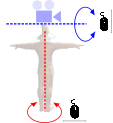
\includegraphics[width=9cm]{kamera_2.png}
\caption{Schemat działania systemu sterowania kamerą}
\end{figure}

\begin{lstlisting}[caption={Obrót kamery za pomocą myszy}]
if (!photonView.isMine) return;
if (!stopCamera)
{
    Camera.main.transform.Rotate(new Vector3(-Input.GetAxis("Mouse Y") * rotationSensitivity * Time.deltaTime, 0, 0));
    rb.transform.Rotate(new Vector3(0, Input.GetAxis("Mouse X") * rotationSensitivity * Time.deltaTime, 0));
}
\end{lstlisting}

Obrót kamery polega na dodaniu wektora obrotu do odpowiedniej osi kamery, natomiast wielkość wektora określona jest przez wartość chwilowego przesunięcia myszy, skalowanego parametrem \textit{rotationSensivity} w celu określenia czułości myszki. Parametr \textit{Time.deltaTime} zwraca czas od ostatniej wyrenderowanej klatki, co pozwala na uzyskanie jednolitej czułości myszki bez względu na ilość generowanych klatek na sekundę.

\subsection{Celownik}

Aby ułatwić celowanie w przeciwników oraz interakcję z otoczeniem umieściliśmy w grze celownik, który w dalszym etapie tworzenia gry zmienia kolor informując o możliwej interakcji.

Celownik jest obiektem 2D nałożonym na ekran w formie \textit{Sprite'a}. Sprite'y to 2-wymiarowe, wcześniej przygotowane obiekty graficzne. W naszym wypadku posłużyliśmy się bezstratnym formatem PNG.

Do sceny został dodany obiekt, na który nałożyliśmy komponenty \name{Canvas} oraz \name{CanvasScaler}. Nakładają one na ekran dwuwymiarowe płótno oraz pozwalają na skalowane go względem podanej rozdzielczości referencyjnej. Wewnątrz takiego płótna można umieszczać obrazy, elementy interfejsu oraz różnego rodzaju wskaźniki (np. Pasek postępu życia bohatera).

\begin{figure}[H]
\center
\includegraphics[width=5cm]{celownik_1.png}
\caption{Konfiguracja płutna 2D do wyświetlania interfejsu gry}
\end{figure}

Wewnątrz płótna został umieszczony obrazek (komponent \name{Image}) celownika, wyrównany do środka ekranu.

\begin{figure}[H]
\center
\includegraphics[width=6cm]{celownik_2.png}
\caption{Gotowy celownik gracza}
\end{figure}
\section{Fizyka}\label{sec:fizyka}

Ważnym elementem gry jest fizyka, aby postaci mogły poruszać się, podskakiwać i reagować na kolizje.

Podstawowym komponentem zapewniającym obliczenia fizyczne jest \name{Rigidbody}. Komponent ten przyjmuje parametry takie jak wartość masy, tarcia, czy wyłączenie grawitacji.

Aby zdarzenia fizyczne mogły mieć miejsce, na elementy otoczenia oraz samą postać gracza nałożone powinny zostać komponenty \name{Collider}. Są to obszary określające granice kolizji. Mogą one mieć kształt kapsuły, sześcianu, bądź uproczczonego modelu samego obiektu. Pozwalają one silnikowi gry na przyspieszenie obliczeń i płynne reakcje na zdarzenia kolizji.

\begin{figure}[H]
\center
\includegraphics[width=6cm]{fizyka_1.png}
\caption{Przykład -- collider mapy terenu}
\end{figure}

W przypadku postaci poruszających się po mapie, zablokowane zostały obroty we wszystkich osiach (parametr \name{Freeze Rotation} komponentu Rigidbody), dzięki czemu nie przewracają się one na bok przy nierównościach terenu i kolizjach z otoczeniem. Zdarzenia fizyczne wyliczane są jedynie w pionie (spadanie, skok itp.).

\subsection{Mechanika skakania postaci}

Mając już zaimplementowaną fizykę, dodaliśmy możliwość skoku. Utworzona została metoda \textit{jump()}, która dodaje do zdarzeń fizycznych naszej postaci siłę w kierunku pionowym o wektorze ustalonym parametrem \textit{jumpPower}. Natomiast na podstawie kolizji z terenem ustalane jest, czy postać stoi na ziemi, dzięki czemu nie można wykonać kolejnego skoku będąc już w powietrzu.
\\
\begin{lstlisting}[caption={Fragment algorytmu skoku postaci}]
void Start()
{
    rb = GetComponent<Rigidbody>();
    anim = GetComponent<Animator>();
}

void jump()
{
    if (onGround)
    {
        onGround = false;
        rb.AddRelativeForce(new Vector3(0, jumpPower, 0));
        anim.SetTrigger("Jump");
    }
}

void OnTriggerEnter(Collider other)
{
    onGround = true;
}
\end{lstlisting}
\subsection{Animacje}
Jednym z głównych komponentów na obiekcie jest Animator.
To dzięki niemu postacie odpowiednio poruszają się podczas zmieniania swojej pozycji lub ataku.
Animator jest odpowiedzialny za wszystkie animacje odgrywane przez nasze postaci, zarówno te sterowane przez komputer, jak i graczy.

Składa się on z dwóch ważnych elementów. Jednym z nich jest kontroler, który odpowiada za wszystkie przejścia pomiędzy naszymi animacjami. Odbiera on parametry, które na bieżąco aktualizowane są przez odpowiednie skrypty zaimplementowane dla danego obiektu. Wykrywają one wszystkie sygnały z urządzeń wejścia, odbierają informacje od innych graczy, postaci niekontrolowanych przez użytkowników oraz otoczenia.

Ważną kwestią jest odpowiednie zaprogramowanie kontrolera, gdyż na jego podstawie postać będzie odpowiednio reagować i przemieszczać się. Jeśli jeden z warunków zawiedzie nasz gracz może pozostać w fazie ataku, która nigdy się nie skończy, przez co będzie blokowała wszystkie inne ruchy dla danej postaci.

Podstawą w kontrolerze są stany, a ich głównym parametrem jest Motion. Zawiera informacje o animacji, która ma się wykonać, gdy postać znajduje się w określonym momencie.

Żeby postać mogła przejść z jednego stanu na drugi niezbędne są transakcje. To na nich ustalamy, na jakie parametry oraz ich wartości ma dojść do zmiany animacji. 

Zwykłe stany posiadają jednak jedną znaczącą wadę, brak płynnych przejść pomiędzy poszczególnymi animacjami. Postać w jednym momencie po prostu zmienia animacje na kolejną, co bardzo psuje efekt wizualny. Aby uniknąć tego w naszym projekcie użyliśmy bardziej zaawansowanej opcji – Blend Tree.

Są to o wiele bardziej rozbudowane stany, które pozwalają na płynne przejścia pomiędzy animacjami oraz łączenie ich. Dzięki czemu nasza postać może połączyć np. bieg w przód z poruszaniem się na boki. Daje to również odczucie, jakby nasza postać posiadała o wiele więcej animacji niż rzeczywiście ma zaimplementowanych.

W Blend Tree możemy wykorzystać również stopniowe zwiększanie się naszych parametrów, co można doskonale zobaczyć w momencie, gdy nasz użytkownik zdecyduje się na sterowanie kontrolerem z gałkami analogowymi, które są czułe na siłę nacisku. Im bardziej gracz będzie przesuwał analog w przód, tym bardziej nasza postać będzie się pochylać i przechodzić płynnie do pełnego sprintu.

\section{Poruszanie bohaterów}

Poruszanie bohaterów działa na podobnej zasadzie jak mechanika skoku. Do zdarzeń fizycznych bohatera dodawana jest siła o wektorze skierowanym w kierunku określonym przez wciskany klawisz (W, S, A lub D).

W przypadku chodzenia, animacja zależna jest od kierunku, w którym porusza się postać (cofanie, chodzenie bokiem).

Dodatkowym elementem mechaniki poruszania jest bieg, który aktywowany jest poprzez wciśnięcie lewego klawisza Shift.

\begin{lstlisting}[caption={Fragment kodu mechaniki biegania -- reakcja na wciśnięcie klawisza \name{W}}]
run = Input.GetKey(KeyCode.LeftShift);
anim.SetBool("Sprint", run);
float speed = run ? runSpeed : walkSpeed;

...

if (Input.GetKey(KeyCode.W))
{
    rb.AddRelativeForce(Vector3.forward * speed, ForceMode.VelocityChange);
}
\end{lstlisting}
\section{Poruszanie postaci wrogów}\label{sec:poruszanie_wrogow}

Poruszanie wrogów odbywa się autonomicznie. Droga jest wyliczana, a koordynacje postaci zmieniane są zgodnie z wyliczoną drogą, dzięki czemu postacie wroga przemieszczają się płynnie w kierunku zdefiniowanego celu.

Unity posiada mechanizm wyznaczania dróg na mapie terenu (więcej informacji na ten temat w dziale~\ref{sec:budowa_terenu} na stronie \pageref{sec:budowa_terenu}). Aby móc z niego skorzystać, dodaliśmy do postaci wroga agenta nawigacji \name{NavAgent}. Jest to komponent zajmujący się obliczeniami drogi i zarządzaniem przemieszczeniem i obrotem postaci w czasie. Podstawowym parametrem jest 3-wymiarowy wektór określający docelową pozycję, silnik gry zajmuje się wyliczeniem trasy prowadzącej do punktu.

Mechanika wrogów polega na wyszukiwaniu najbliżej znajdującej się postaci gracza, a następnie ustaleniu jej jako cel podążania wroga. W momencie, gry wróg znajduje się odpowiednio blisko, rozpoczyna atak.
\\
\begin{lstlisting}[caption={Algorytm zwracający wskaźnik do obiektu znajdującego się najbliżej, przy określonym maksymalnym promieniu poszukiwań}]
GameObject findNearestPlayer(float maxDistance)
{
    GameObject[] players = GameObject.FindGameObjectsWithTag("Player");
    GameObject nearestPlayer = null;
    float distance = maxDistance;
    foreach (GameObject player in players)
    {
        float distanceFromEnemy = Vector3.Distance(player.transform.position, transform.position);
        if (distanceFromEnemy < distance)
        {
            distance = distanceFromEnemy;
            nearestPlayer = player;
        }
    }
    return nearestPlayer;
}
\end{lstlisting}

\begin{figure}[H]
\center
\includegraphics[width=\textwidth]{poruszanie_wrogow_1.png}
\caption{Obszary interakcji postaci wroga}
\end{figure}

W przypadku, gdy wróg ``widzi,, postać gracza, jest w jego stronę stale odwrócony. Służy do tego algorytm, który najpierw wylicza kierunek w postaci wektora wartości w skalu 0.0f..1.0f w przestrzeni 3D, a następnie zamienia wektor na kąt, do którego stopniowo dąży. Daje to efekt płynnego obracania postaci wroga z możliwością dostosowania prędkości obrotu, aby ruchy wyglądały naturalnie, a wróg dawał możliwość np. zajścia go od tyłu.
\\
\begin{lstlisting}[caption={Algorytm obracania postaci wroga w kierunku gracza}]
private void rotateTowards(Transform target)
{
    Vector3 direction = (target.position - transform.position).normalized;
    Quaternion lookRotation = Quaternion.LookRotation(direction);
    transform.rotation = Quaternion.Slerp(transform.rotation, lookRotation, Time.deltaTime * 5);
}
\end{lstlisting}
\section{Umiejętności Bohaterów}
Zgodnie z naszymi założeniami każdy bohater miał być unikalny i odgrywać ważną rolę w całej rozgrywce. Wszystkich nadaliśmy różne umiejętności, a każda z nich jest niezbędna, by wspólnie ukończyć grę.

\subsection{Wojownik}

Wojownik słynie z ogromnej siły, jego zadaniem jest rozprawianie się z jak największą ilością przeciwników. Do jego postaci napisaliśmy skrypt, który pobiera listę obiektów znajdujących się w jego obrębie a następnie każdemu z nich odbiera życie. Skrypty dodawane są do postaci na podobnej zasadzie, jak \name{Komponenty}. W jednej z klatek animacji uderzenia mieczem ustawiliśmy tzw. \name{Trigger}, który uruchamia odpowiednie zdarzenie. Każda z postaci znajdujących się na planszy posiada specjalny \name{Tag}, jest to dodatkowa informacja o obiekcie w postaci ciągu znaków, w wypadku wroga jest to \textit{Enemy}. Siła rażenia zależna jest od rodzaju ataku (Wojownik posiada 2 rodzaje ataku - standardowy szybki oraz silny, który jednak trwa nieco dłużej).
\\
\begin{lstlisting}[caption={Algorytm zadawania obrażeń wrogom}]
// HitEvent is animation triggered method
void HitEvent(int type)
{
    if (!photonView.isMine) return;

    Collider[] hitColliders = Physics.OverlapSphere(transform.position, attackDistance);
    foreach (var enemyCollider in hitColliders)
    {
        if (enemyCollider.tag == "Enemy")
        {
            float damageValue = 0.0f;
            switch (type)
            {
                case 0: damageValue = 20.0f; break;
                case 1: damageValue = 50.0f; break;
            }
            enemyCollider.gameObject.GetPhotonView().RPC("damage", PhotonTargets.All, damageValue);
        }
    }
}
\end{lstlisting}


\subsection{Mag}

Mag posiada umiejętność podnoszenia przedmiotów, którą możemy wykorzystać na dwa sposoby. Jednym z nich jest pokonywanie przeszkód, drugim atak. Specjalny skrypt umieszczony w komponentach wykorzystuje celownik, za którym podąża kamera. Gdy najedziemy celownikiem na obiekt o odpowiednim oznaczeniu, możemy go podnieść. Gracz może obracać przedmiot wokół własnej osi, oddalać go od siebie i przybliżać. Przy pomocy odpowiedniego przycisku może również rzucić trzymanym przedmiotem w przeciwnika. Dzięki wykorzystaniu grawitacji i kolizji z danymi przedmiotami możemy w ten sposób zabrać życie naszym przeciwnikom.

Aby odnaleźć interesujący nas obiekt, tworzymy wiązkę (\textit{Ray}), przechodzącą z pozycji kamery przez środek ekranu, gdzie znajduje się celownik, a następnie pobieramy listę wszystkich obiektów, które ta wiązka przecina, przy zadanej maksymalnej odległości. Następnie iterujemy poprzez wszystkie znalezione obiekty, i gdy znajdziemy obiekt posiadający tag \textit{Holdable}, wyłączamy grawitację tego obiektu, wyliczamy odległość od niego, a następnie pobieramy jego wskaźnik do zmiennej globalnej, w celu możliwości manipulowania tym obiektem:
\\
\begin{lstlisting}[caption={Algorytm wykrywania obiektów w obrębie Maga, które mogą zostać przeniesione}]
ray = Camera.main.ScreenPointToRay(new Vector3(Screen.width / 2, Screen.height / 2));
hits = Physics.RaycastAll(ray);
foreach (var hit in hits)
{
    if (hit.transform.gameObject.tag == "Holdable" && hit.distance < objectDistanceMax)
    {
        turnSpecialCrosshair(true);

        if (Input.GetMouseButtonDown(0) && holdedThing == null)
        {
            holdedThing = hit.transform.gameObject;
            objectDistance = Mathf.Clamp(hit.distance, colliderSize(holdedThing) / 2 + objectDistanceMin, objectDistanceMax);
            holdedThing.GetComponent<PhotonView> ().RequestOwnership ();
            photonView.RPC("setGravity", PhotonTargets.All, hit.transform.gameObject.GetComponent<PhotonView>().viewID, false);
            break;
        }
    } else
    {
        turnSpecialCrosshair(false);
    }
}
\end{lstlisting}

Po wykryciu obiektu, który da się przenieść, zmienia się również kolor wskaźnika (na zasadzie podmiany grafiki celownika). Nie wdrażając się we wszystkie szczegóły (oddalanie, przybliżanie, rzucanie - są to kolejne manipulacje obiektem), fragment kodu przemieszczania obiektów wylicza punkt w przestrzeni 3D oddalony o odpowiednią wartość od widoku kamery, a następnie na tej podstawie wylicza trójwymiarowy wektor prędkości, dzięki czemu przenoszony obiekt dąży w każdej z osi do docelowego punktu:
\\
\begin{lstlisting}[caption={Algorytm przenoszenia obiektów}]
// Moving object in space
if (holdedThing != null)
{
    // Get point in front of camera
    var newObjectPosition = ray.GetPoint(objectDistance);

    // Move holded thing to new destination in front of camera
    var holdedThingDestination = Vector3.ClampMagnitude((newObjectPosition - holdedThing.transform.position) * objectMoveSpeed, objectMoveSpeed);
    holdedThing.GetComponent<Rigidbody>().velocity = holdedThingDestination;
...
\end{lstlisting}

Wartość prędkości podążania obiektu za punktem docelowym jest ustawiona z góry i dopasowana tak, aby przenoszony obiekt sprawiał wrażenie delikatnej bezwładności.


Łotr jest przebiegły, potrafi pozyskiwać informacje oraz dostrzega znacznie więcej niż inni. Posiada skrypt, który umożliwia mu rozmowę z innymi osobami, która udzielają mu cennych informacji, gdy tylko znajdzie się w odpowiedniej odległości. Może też wyszukiwać przedmioty, które pozostają niewidoczne dla pozostałych graczy.

\subsection{Multiplayer}
Ostatnim elementem implementacji naszego projektu był system Multiplayer. Stworzyliśmy Menadżera naszej sieci, który odpowiednio łączył graczy z serwerem i kontrolował ilość osób w danej rozgrywce. Napotkaliśmy jednak wiele problemów, gdyż wszystkie funkcje były wykonywane tylko lokalnie u danego gracza.

Jeśli wojownik atakował, potwory traciły życie, lecz ta informacja wyświetlała się tylko u jednego z graczy. To samo miało miejsce w przypadku animacji i poruszanych obiektów.

Z drugiej strony pojawił się problem sterowania daną postacią, gdyż Unity nie odróżniało, do którego gracza należy dana postać i jeden z trzech graczy poruszał wszystkimi bohaterami.

Najpierw zajęliśmy się problemem poruszania postaciami. Photon nadaje każdemu obiektowi posiadającemu komponent PhotonView odpowiednie ID. W skryptach, które odczytywały wszystkie sygnały z wejścia. Mogliśmy wykorzystać ten fakt i przed wykonaniem jakiejkolwiek operacji sprawdzaliśmy, czy dany widok, który wyświetla dany gracz jest zgodny z jego numerem ID. 

Do rozwiązania problemu z przesyłaniem animacji oraz pozycji pomiędzy graczami użyliśmy na obiektach komponentów PhotonRigidBodyView oraz PhotonAnimatorView, które musiały zostać połączone z komponentem PhotonView przechowującym nasze unikalne ID.

Finalnym krokiem było poprawne wykonywanie pozostałych funkcji, takie jak przenoszenie przedmiotów, atakowanie potworów, czy rozmowa z NPC.
Rozwiązanie w tym wypadku zaimplementowaliśmy w naszym Menadżerze połączeń. 
Domyślnie wszystkie skrypty, które kolidowały pomiędzy postaciami zostały na obiektach wyłączone. W momencie, gdy użytkownik łączy się do gry, wszystkie komponenty zostają aktywowane konkretnie dla danego obiektu. Dzięki tym zabiegom Framework odróżnia, który gracz wywołał daną funkcję oraz synchronizuje wszystkie dane u pozostałych użytkowników.


\chapter{Bibliografia}
\section{Bibliografia}

Photon Documentation https://doc-api.photonengine.com/en/pun/current

Unity Documentation https://docs.unity3d.com/Manual/index.html

C Sharp Documentation https://msdn.microsoft.com/en-us/library/67ef8sbd.aspx

Stack Overflow https://stackoverflow.com

Mixamo https://www.mixamo.com
\end{document}
